\section{Simon}
\subsection{Overview}
\begin{frame}{Simon: Overview}
	\begin{itemize}
	  \item Programming language
	  \item Hardware/software architecture
	  \item Physics implementation
	\end{itemize}
\end{frame}

\subsection{Programming Language}
\begin{frame}{Programming Language}
	\begin{itemize}
	  \item Choosing a programming language
	  \begin{itemize}
	  	\item NXC
	  	\item Pros
	  	\begin{itemize}
	  	  \item Low level 
	  	  \item C-like
	  	\end{itemize}
	  	\item Cons
	  	\begin{itemize}
	  	  \item Bad documentation
	  	  \item No control over the scheduler
	  	  \item No unit test environment
	  	  \item No debugger
	  	\end{itemize}
	  \end{itemize}
	  \item Alternatives
	  \begin{itemize}
	    \item leJos
	    \item ROBOTC
	  \end{itemize}
	\end{itemize}
\end{frame}

\subsection{Hardware/Software Architecture}
\begin{frame}{Hardware/Software Architecture}
\begin{onlyenv}
\only<1>{
\begin{itemize}
  \item Hardware Architecture 
\end{itemize}
	\begin{figure}[H]
  		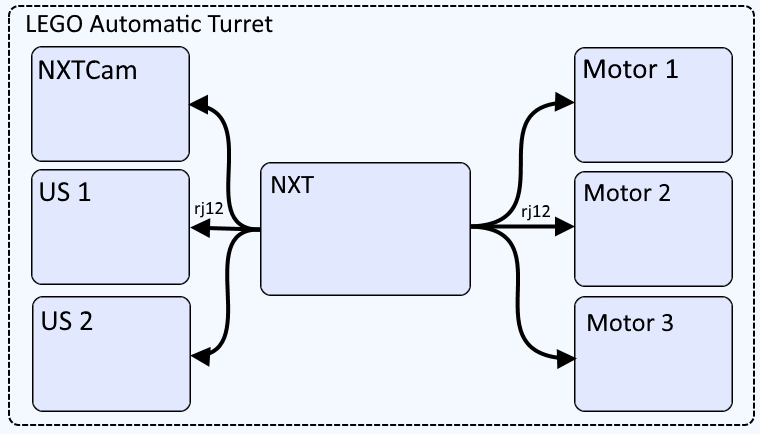
\includegraphics[scale=0.45]{figures/HARCH.png}
	\end{figure}
	}
\only<2>{
\begin{itemize}
  \item Software Architecture
  \item Calls through the software
\end{itemize}
	\begin{figure}[H]
		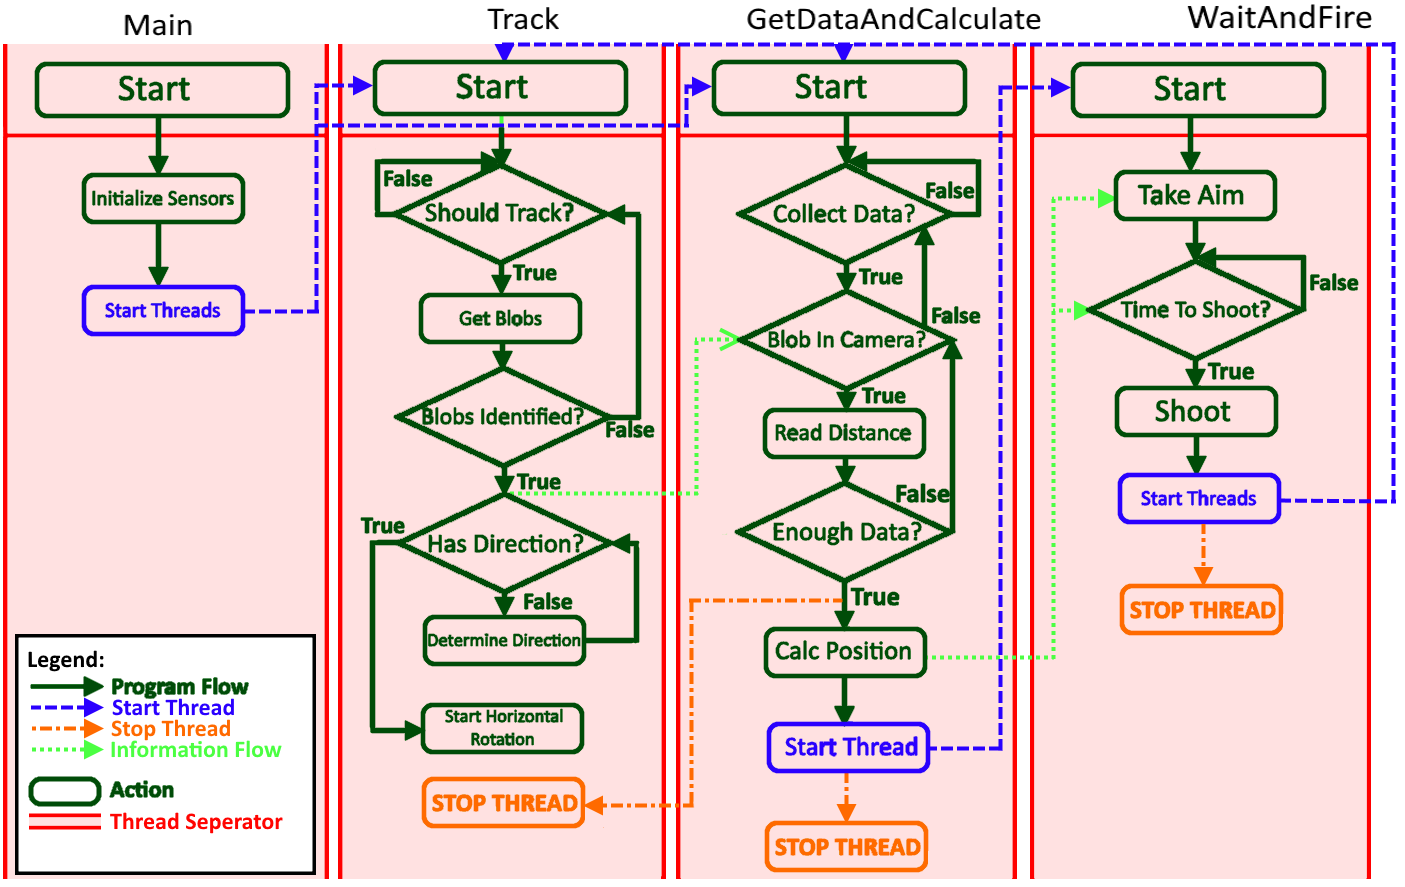
\includegraphics[scale=0.26]{figures/SequenceDiagram.png}
	\end{figure}
}
\end{onlyenv}
\end{frame}

\subsection{Physics Implementation}
\begin{frame}{Physics Implementation}

\begin{figure}[H]
	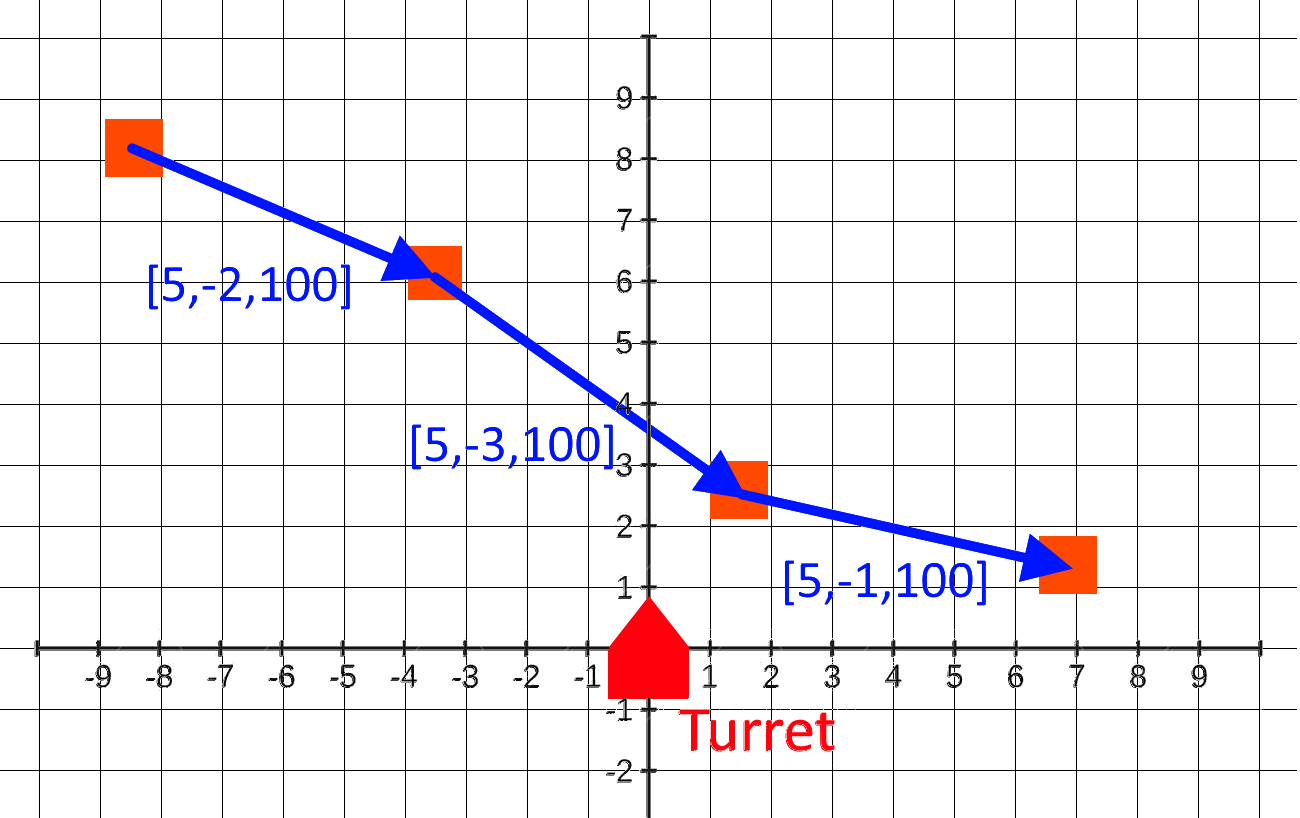
\includegraphics[scale=0.25]{figures/FPosCalc2.png}
\end{figure}

\end{frame}

\begin{frame}[fragile]{Physics Implementation}
\begin{center}
\begin{minipage}[H]{0.9\linewidth}
 \begin{lstlisting}
PosData CalcFuturePos(DirectionVector vector, unsigned long time){
   PosData futurePosition;
   float tanInput = 0;
   futurePosition.xPos = vector.xPos + vector.speedX * time;
   futurePosition.yPos = vector.yPos + vector.speedY * time;
   futurePosition.time = CurrentTick() + time;

   tanInput = futurePosition.yPos / futurePosition.xPos;
   if(futurePosition.xPos >= 0)
        futurePosition.angle = 90+(atand(tanInput))*(-1);
   else
        futurePosition.angle = (90-(atand(tanInput))*(-1))*(-1);
   
   return futurePosition;
}
 \end{lstlisting} 
\end{minipage}
\end{center}
\end{frame}